\documentclass[10pt,a4paper]{amsart}
\usepackage[margin=19mm]{geometry}
\usepackage{amsmath,amssymb,mathtools}
\usepackage[scr=rsfs,cal=euler]{mathalfa}
\usepackage{xfrac}
\usepackage[unicode,hidelinks,bookmarks=false]{hyperref}
\newcommand{\ie}{i.e.\ }
\newcommand{\cf}{cf.\ }
\newcommand{\resp}{respectively\ }
\newcommand{\Subsection}{\subsection}
\providecommand{\nobreakdash}{\nobreak\hbox{-}}
\setlength{\emergencystretch}{2em}
\multlinegap0pt
\usepackage{tikz}
\usepackage{float}
\usepackage{mathtools}
\usepackage{amssymb}
\usepackage{bm}
\usepackage[shortlabels]{enumitem}
\usepackage{xcolor}
\newtheorem{lemma}{Lemma}
\usepackage{cleveref}
\crefname{lemma}{Lemma}{Lemmas}
\newcommand{\NN}{\mathbb{N}}
\newcommand{\R}{\RR}
\newcommand{\RR}{\mathbb{R}}
\DeclareMathOperator*{\argmin}{argmin}
\title{\huge Breakdown properties of optimal transport maps: general transportation costs}
\author{Alberto Gonz{\'a}lez-Sanz \and Marco Avella Medina}
\date{Source: arXiv:2603.16005v1 (CC BY 4.0)}
\begin{document}
\maketitle

\noindent\emph{Source and licence.} \huge Breakdown properties of optimal transport maps: general transportation costs. Version arXiv:2603.16005v1 (CC BY 4.0), distributed by arXiv under the Creative Commons Attribution 4.0 International licence, http://creativecommons.org/licenses/by/4.0/, as recorded in the arXiv licence metadata for this exact version and shown on the abstract page https://arxiv.org/abs/2603.16005v1. Full licence notice: \texttt{licenses/arxiv-2603.16005-CC-BY-4.0.txt}.\par\smallskip

\noindent\textit{Editorial scope.} Counted unit: the article's lemma lem:finite\_sample\_UB (source0.tex lines 667--679). The article's complete original proof of it is delivered with it (source0.tex lines 681--807, one \texttt{proof} environment of 127 lines). No mathematics is written, repaired or re-derived: the statement and the proof are the article's own lines, in the article's own notation, and no retained line is substituted or re-flowed.  Retained uncounted as the source-local context the proof needs: lines 626--647.  Nothing was omitted from any retained span, so the package carries no omission record.  No retained line contains a citation, so the wrapper carries no bibliography and no bibliography entry.  The retained lines contain the article's own diagram code, which the wrapper typesets with the standard tikz packages; no image file is delivered and the package declares no asset dependency.  Editorial formatting only, in addition: an AMS \texttt{amsart} preamble that restates the article's own declarations and macros used by the retained lines, namely the environments \texttt{lemma} on separate counters, together with the standard packages those lines need.  The retained environments print in this document as Lemma 1 in order of appearance, whereas the article prints the same items with the numbering of its own full document.  The complete native source of the article as distributed in the arXiv e-print for this exact version is bundled unchanged as \texttt{sources/196512/source0.tex}.
\begin{lemma}\label{lemma:discrete-upper}
    Fix $j\in \{1, \dots, n\}$, and $v\in \mathbb{S}^{d-1}$.  
%
Relabel  the reference sample $u^{(n)}=\{u_1, \dots, u_{n}\}= \{ u_{(1)}, \dots, u_{(n)}\}$ in such a way that for some $\ell\in \{1, \dots, n\}$,  $u_{(\ell)}= u_j$, 
$$ \{u_i\}_{i=1}^{\ell}= \{ x\in \mathbb{R}^d: \langle v, x-u_j\rangle \leq  0\} \cap u^{(n)}. $$
Fix $z_0\in \R^d$. For each $k\in \NN$ and $m\in \NN$, 
    define the measure 
    \begin{equation}\label{eq:def-nu-zeta}
        \nu_{k,v,m}=\frac{m}{n} \delta_{ z_{k,v,m}} + \frac{1}{n} \sum_{i=m+1}^n \delta_{T_{Q_n\to P_n}(u_{(i)})} , \quad \text{where}\quad z_{k,v,m} = u_{(\ell)} - \nabla h^{*}(z_0+k\, v). 
    \end{equation} Then the following hold: 

\begin{enumerate}
    \item  If   $ T_{Q_n\to \nu_{k,v,m}}(u_{(r)})=z_{k,v,m} $ for $k\in \NN$ large enough and some $r\geq \ell+1$, then
    $$ \text{$\| T_{Q_n\to \nu_{k,v,m}}(u_{j} )\|\to \infty  $ as $k\to \infty$.}$$
     
    \item If $m\geq \ell$, then $\| T_{Q_n\to \nu_{k,v,m}}(u_{j} )\|\to \infty  ,$ as $k\to \infty$. 
    \item ${\rm BP}({ T}_{Q_n\to P_n}(u_j), P_n) \leq  \frac{\ell}{n}$.
\end{enumerate}



\end{lemma}

\begin{lemma}[Finite sample upper bound]\label{lem:finite_sample_UB}
For every $j=1, \dots, n$, 
\begin{equation}
    \label{eq:discrete-BP-proof}
     {\rm BP}({ T}_{Q_n\to P_n}(u_j), P_n) \leq  {\rm TD}(u_j;Q_n) .
\end{equation}
If, furthermore, $u^{(n)}=\{u_1, \dots, u_n\}$ is in general position, then 
\begin{equation}
    \label{eq:General-Position-proof}
    {\rm BP}({ T}_{Q_n\to P_n}(u_j), P_n) \leq  
{\rm TD}^{-}(u_j;Q_n)+\frac{1}{n}.
\end{equation}
\end{lemma}

\begin{proof}
In order to prove \eqref{eq:discrete-BP-proof}, we apply \Cref{lemma:discrete-upper}~(iii) to the vector 
%
$$v_*\in \argmin_{v\in \mathbb{S}^{d-1}} Q_n (\{ x: \langle v, x-u_j\rangle \leq  0\}).$$
%
and  $\ell=\sum_{i=1}^n {\bf 1}_{\langle v_*, u_i-u_j\rangle \leq  0}$. Since $\ell/n={\rm TD}(u_j; Q_n)$, we have found the upper bound \eqref{eq:discrete-BP-proof}. 

 To prove \eqref{eq:General-Position-proof}, define 
 %
 $$w\in \argmin_{v\in \mathbb{S}^{d-1}} Q_n (\{ x: \langle v, x-u_j\rangle <  0\}).$$
 %
 We will apply \cref{lemma:discrete-upper} to a  continuous perturbation of  $w$ defining a hyperplane containing exactly one more point than $\{ x: \langle w, x-u_j\rangle <  0\}$. The intuition for this is simple: the general position assumption implies that no more than 2 points can lie in the same line. 
 \begin{figure}[h!]
    \centering
    


\tikzset{every picture/.style={line width=0.75pt}} %

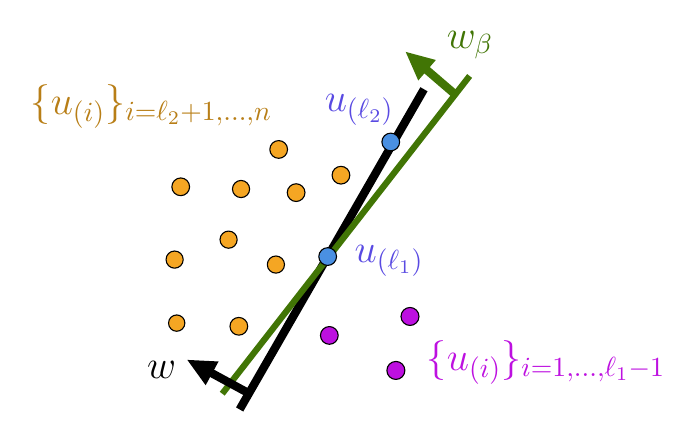
\begin{tikzpicture}[x=0.6pt,y=0.6pt,yscale=-1,xscale=1]
%

%
\draw [color={rgb, 255:red, 0; green, 0; blue, 0 }  ,draw opacity=1 ][line width=3]    (375.83,42.08) -- (264.83,234.92) ;
%
\draw  [fill={rgb, 255:red, 245; green, 166; blue, 35 }  ,fill opacity=1 ] (259,184.83) .. controls (259,181.89) and (261.39,179.5) .. (264.33,179.5) .. controls (267.28,179.5) and (269.67,181.89) .. (269.67,184.83) .. controls (269.67,187.78) and (267.28,190.17) .. (264.33,190.17) .. controls (261.39,190.17) and (259,187.78) .. (259,184.83) -- cycle ;
%
\draw  [fill={rgb, 255:red, 74; green, 144; blue, 226 }  ,fill opacity=1 ] (350.5,73.83) .. controls (350.5,70.89) and (352.89,68.5) .. (355.83,68.5) .. controls (358.78,68.5) and (361.17,70.89) .. (361.17,73.83) .. controls (361.17,76.78) and (358.78,79.17) .. (355.83,79.17) .. controls (352.89,79.17) and (350.5,76.78) .. (350.5,73.83) -- cycle ;
%
\draw  [fill={rgb, 255:red, 189; green, 16; blue, 224 }  ,fill opacity=1 ] (313.5,190.33) .. controls (313.5,187.39) and (315.89,185) .. (318.83,185) .. controls (321.78,185) and (324.17,187.39) .. (324.17,190.33) .. controls (324.17,193.28) and (321.78,195.67) .. (318.83,195.67) .. controls (315.89,195.67) and (313.5,193.28) .. (313.5,190.33) -- cycle ;
%
\draw  [fill={rgb, 255:red, 245; green, 166; blue, 35 }  ,fill opacity=1 ] (293.5,104.33) .. controls (293.5,101.39) and (295.89,99) .. (298.83,99) .. controls (301.78,99) and (304.17,101.39) .. (304.17,104.33) .. controls (304.17,107.28) and (301.78,109.67) .. (298.83,109.67) .. controls (295.89,109.67) and (293.5,107.28) .. (293.5,104.33) -- cycle ;
%
\draw [color={rgb, 255:red, 65; green, 117; blue, 5 }  ,draw opacity=1 ][line width=2.25]    (403.33,34.08) -- (254.33,225.42) ;
%
\draw  [fill={rgb, 255:red, 74; green, 144; blue, 226 }  ,fill opacity=1 ] (312.5,142.83) .. controls (312.5,139.89) and (314.89,137.5) .. (317.83,137.5) .. controls (320.78,137.5) and (323.17,139.89) .. (323.17,142.83) .. controls (323.17,145.78) and (320.78,148.17) .. (317.83,148.17) .. controls (314.89,148.17) and (312.5,145.78) .. (312.5,142.83) -- cycle ;
%
\draw [line width=3]    (238.61,207.95) -- (270,225) ;
\draw [shift={(233.33,205.08)}, rotate = 28.51] [fill={rgb, 255:red, 0; green, 0; blue, 0 }  ][line width=0.08]  [draw opacity=0] (16.97,-8.15) -- (0,0) -- (16.97,8.15) -- cycle    ;
%
\draw [color={rgb, 255:red, 65; green, 117; blue, 5 }  ,draw opacity=1 ][line width=3]    (369.38,23.49) -- (394.5,45.08) ;
\draw [shift={(364.83,19.58)}, rotate = 40.68] [fill={rgb, 255:red, 65; green, 117; blue, 5 }  ,fill opacity=1 ][line width=0.08]  [draw opacity=0] (16.97,-8.15) -- (0,0) -- (16.97,8.15) -- cycle    ;
%
\draw  [fill={rgb, 255:red, 245; green, 166; blue, 35 }  ,fill opacity=1 ] (224,100.83) .. controls (224,97.89) and (226.39,95.5) .. (229.33,95.5) .. controls (232.28,95.5) and (234.67,97.89) .. (234.67,100.83) .. controls (234.67,103.78) and (232.28,106.17) .. (229.33,106.17) .. controls (226.39,106.17) and (224,103.78) .. (224,100.83) -- cycle ;
%
\draw  [fill={rgb, 255:red, 245; green, 166; blue, 35 }  ,fill opacity=1 ] (283,78.33) .. controls (283,75.39) and (285.39,73) .. (288.33,73) .. controls (291.28,73) and (293.67,75.39) .. (293.67,78.33) .. controls (293.67,81.28) and (291.28,83.67) .. (288.33,83.67) .. controls (285.39,83.67) and (283,81.28) .. (283,78.33) -- cycle ;
%
\draw  [fill={rgb, 255:red, 245; green, 166; blue, 35 }  ,fill opacity=1 ] (253,132.67) .. controls (253,129.81) and (255.31,127.5) .. (258.17,127.5) .. controls (261.02,127.5) and (263.33,129.81) .. (263.33,132.67) .. controls (263.33,135.52) and (261.02,137.83) .. (258.17,137.83) .. controls (255.31,137.83) and (253,135.52) .. (253,132.67) -- cycle ;
%
\draw  [fill={rgb, 255:red, 245; green, 166; blue, 35 }  ,fill opacity=1 ] (281.5,147.67) .. controls (281.5,144.81) and (283.81,142.5) .. (286.67,142.5) .. controls (289.52,142.5) and (291.83,144.81) .. (291.83,147.67) .. controls (291.83,150.52) and (289.52,152.83) .. (286.67,152.83) .. controls (283.81,152.83) and (281.5,150.52) .. (281.5,147.67) -- cycle ;
%
\draw  [fill={rgb, 255:red, 245; green, 166; blue, 35 }  ,fill opacity=1 ] (220.5,144.67) .. controls (220.5,141.81) and (222.81,139.5) .. (225.67,139.5) .. controls (228.52,139.5) and (230.83,141.81) .. (230.83,144.67) .. controls (230.83,147.52) and (228.52,149.83) .. (225.67,149.83) .. controls (222.81,149.83) and (220.5,147.52) .. (220.5,144.67) -- cycle ;
%
\draw  [fill={rgb, 255:red, 245; green, 166; blue, 35 }  ,fill opacity=1 ] (260.5,102.17) .. controls (260.5,99.31) and (262.81,97) .. (265.67,97) .. controls (268.52,97) and (270.83,99.31) .. (270.83,102.17) .. controls (270.83,105.02) and (268.52,107.33) .. (265.67,107.33) .. controls (262.81,107.33) and (260.5,105.02) .. (260.5,102.17) -- cycle ;
%
\draw  [fill={rgb, 255:red, 245; green, 166; blue, 35 }  ,fill opacity=1 ] (320.5,93.83) .. controls (320.5,90.89) and (322.89,88.5) .. (325.83,88.5) .. controls (328.78,88.5) and (331.17,90.89) .. (331.17,93.83) .. controls (331.17,96.78) and (328.78,99.17) .. (325.83,99.17) .. controls (322.89,99.17) and (320.5,96.78) .. (320.5,93.83) -- cycle ;
%
\draw  [fill={rgb, 255:red, 189; green, 16; blue, 224 }  ,fill opacity=1 ] (362,178.92) .. controls (362,175.93) and (364.43,173.5) .. (367.42,173.5) .. controls (370.41,173.5) and (372.83,175.93) .. (372.83,178.92) .. controls (372.83,181.91) and (370.41,184.33) .. (367.42,184.33) .. controls (364.43,184.33) and (362,181.91) .. (362,178.92) -- cycle ;
%
\draw  [fill={rgb, 255:red, 189; green, 16; blue, 224 }  ,fill opacity=1 ] (353.5,211.42) .. controls (353.5,208.43) and (355.93,206) .. (358.92,206) .. controls (361.91,206) and (364.33,208.43) .. (364.33,211.42) .. controls (364.33,214.41) and (361.91,216.83) .. (358.92,216.83) .. controls (355.93,216.83) and (353.5,214.41) .. (353.5,211.42) -- cycle ;
%
\draw  [fill={rgb, 255:red, 245; green, 166; blue, 35 }  ,fill opacity=1 ] (222,182.92) .. controls (222,180.2) and (224.2,178) .. (226.92,178) .. controls (229.63,178) and (231.83,180.2) .. (231.83,182.92) .. controls (231.83,185.63) and (229.63,187.83) .. (226.92,187.83) .. controls (224.2,187.83) and (222,185.63) .. (222,182.92) -- cycle ;

%
\draw (314.5,43.33) node [anchor=north west][inner sep=0.75pt]  [font=\Large,color={rgb, 255:red, 89; green, 74; blue, 226 }  ,opacity=1 ] [align=left] {$\displaystyle u_{( \ell _{2})}$};
%
\draw (388,5.33) node [anchor=north west][inner sep=0.75pt]  [font=\Large,color={rgb, 255:red, 65; green, 117; blue, 5 }  ,opacity=1 ] [align=left] {$\displaystyle w_{\beta }$};
%
\draw (207.5,204.5) node [anchor=north west][inner sep=0.75pt]  [font=\Large,color={rgb, 255:red, 0; green, 0; blue, 0 }  ,opacity=1 ] [align=left] {$\displaystyle w$};
%
\draw (332.5,134.33) node [anchor=north west][inner sep=0.75pt]  [font=\Large,color={rgb, 255:red, 89; green, 74; blue, 226 }  ,opacity=1 ] [align=left] {$\displaystyle u_{( \ell _{1})}$};
%
\draw (376,191.83) node [anchor=north west][inner sep=0.75pt]  [font=\Large,color={rgb, 255:red, 189; green, 16; blue, 224 }  ,opacity=1 ] [align=left] {$\displaystyle \{u_{( i)}\}_{i=1,\dotsc ,\ell _{1} -1}$};
%
\draw (137.5,37.83) node [anchor=north west][inner sep=0.75pt]  [font=\Large,color={rgb, 255:red, 184; green, 126; blue, 22 }  ,opacity=1 ] [align=left] {$\displaystyle \{u_{( i)}\}_{i=\ell _{2} +1,\dotsc ,n}$};


\end{tikzpicture}
    \caption{ \small Illustration of the geometric argument used in the proof of \Cref{lem:finite_sample_UB}. If $w$   defines a half-space with  border passing through more than one point, then we can find a slight modification  $w_\beta$  defining a half-space with the same number of interior points, but with  border passing only through $u_{(\ell_1)}$.  }
    \label{fig:intuition-lemma-2}
\end{figure}

 Relabel the reference sample $u^{(n)}$ in such a way that for some ${\ell}_1,\ell_2\in \{1, \dots, n\}$,  $u_{(\ell_1)}= u_j$,
 %
\begin{equation}
    \label{eq:setting-general-position}
     \{u_{(i)}\}_{i=1}^{\ell_1-1}= \{ x: \langle w, x-u_{(\ell_1)}\rangle < 0\} \cap u^{(n)} \ \text{and}\   \{u_{(i)}\}_{i=\ell_1}^{\ell_2}= \{ x: \langle w, x-u_{(\ell_1)}\rangle =  0\} \cap u^{(n)}.
\end{equation}
%
Note that by construction
%
\begin{equation}
    \label{eq:ell-1}
   \frac{ \ell_1}{n}=  {\rm TD}^{-}(u_{(\ell_1)};Q_n)+\frac{1}{n}=  {\rm TD}^{-}(u_j;Q_n)+\frac{1}{n}.
\end{equation}
%
 As $u^{(n)}$ is in general position, it follows that $ u_{(\ell_1)}\notin {\rm aff}( \{u_{(i)}\}_{i=\ell_1+1}^{\ell_2})$, where for a set $S$,   ${\rm aff}(S)$  denotes the smallest affine subspace containing $S$. Since  $u^{(n)}$ is in general position,  it follows that ${\rm aff}( \{u_{(i)}\}_{i=\ell_1+1}^{\ell_2})$ has  dimension  at most $d-2$ and  
 %
 $$ {\rm aff}( \{u_{(i)}\}_{i=\ell_1+1}^{\ell_2})\subset  \{ x: \langle w, x-u_{(\ell_1)}\rangle =  0\}. $$ 
 %
 %
 Then there exists $a>0$,  $v_0 \in \mathbb{S}^{d-1} $ orthogonal to $ w$ and such that 
 %
$$ {\rm aff}(\{u_{(i)}\}_{i=\ell_1+1}^{\ell_2})\subset \{  x: \langle  v_0,x-u_{(\ell_1)}  \rangle =a \} \quad {\rm and}\quad u_{(\ell_1)} \in \{  x: \langle v_0, x -u_{(\ell_1)} \rangle =0 \} . $$
%
Define the continuous function 
%
$$ \R^d\times \R \ni (x,\beta)\mapsto f(x,\beta):= \langle    w_\beta, x -u_{(\ell_1)} \rangle, \quad {\rm for }\quad  w_\beta =\frac{w+ \beta v_0}{\|w+ \beta v_0\|}.   $$
%
Note that, for every $\beta>0$, 
%
$$ \{u_{(i)}\}_{i=\ell_1+1}^{\ell_2} \subset  \{  x: f(x,\beta) >0  \} \quad {\rm and}\quad  u_{(\ell_1)} \in \{  x: f(x,\beta) =0  \}, $$
%
while for $\beta=0$ we recover \eqref{eq:setting-general-position}. Therefore,
%
$$ \{u_{(i)}\}_{i=1}^{\ell_1-1} \subset  \{  x: f(x,0) <0  \},  \quad \{u_{(i)}\}_{i=\ell_2+1}^{n} \subset  \{  x: f(x,0)>0  \} $$ 
%
and $ \{u_{(j)}\}_{j=\ell_1}^{\ell_2}$ are the unique elements of the reference sample $u^{(n)}$ in $\{  x: f(x,0) =0  \}$. Since $f$ is continuous, for every $i\leq \ell_1-1$ (resp.~$i\geq \ell_2+1$), there exists $\beta_{(i)}>0$ such that   $u_{(i)} \in \{  x: f(x,\beta) <0  \} $ (resp.~$u_{(i)} \in \{  x: f(x,\beta) >0  \} $) for all $|\beta|\leq \beta_{(i)}$. Taking $\beta_*=\min_{i} \beta_{(i)}$, we conclude that 
%
$$ \{u_{(i)}\}_{i=1}^{\ell_1-1} \subset  \{  x: f(x,\beta_*) <0  \},  \quad  \{u_{(i)}\}_{i=\ell_1+1}^{n} \subset  \{  x: f(x,\beta_*) >0  \}  $$
%
 and $ u_{(\ell_1)}$ is the unique element of the reference sample $u^{(n)}$ in $\{  x: f(x,\beta_*) =0  \}$. Hence we can apply \cref{lemma:discrete-upper} with $v=w_{\beta_*}$ and $m= \ell_1$ and conclude that 
$$  {\rm BP}({ T}_{Q_n\to P_n}(u_j), P_n) \leq  
\frac{\ell_1}{n}={\rm TD}^{-}(u_j;Q_n)+\frac{1}{n}, $$
where the last equality is \eqref{eq:ell-1}. 

\end{proof}

\end{document}
